%====================================================%
% SEZIONE 1: LAVORO DI UNA FORZA
%====================================================%
\begin{question}[ID=1.1, subtitle={Lavoro di una forza costante inclinata di 30°}, tags={lavoro, energia}, difficulty=facile]
Una forza costante $\vec{F}$ di intensità $F = 15\ \text{N}$ agisce su un corpo, inclinata di $30^\circ$ rispetto allo spostamento, e lo sposta di $s = 4\ \text{m}$. Calcola il lavoro compiuto dalla forza.
\begin{solution}
Il lavoro di una forza costante dipende solo dalla componente della forza lungo lo spostamento, cioè da $F\cos\theta$:
\[
W = F\,s\,\cos 30^\circ = 15\cdot 4\cdot \frac{\sqrt{3}}{2} = 30\sqrt{3} \approx \mathbf{52{,}0\ \text{J}}.
\]
La componente perpendicolare della forza non compie lavoro perché non produce spostamento nella propria direzione.
\end{solution}
\end{question}

%-----------------------------------------------%

\begin{question}[ID=1.2, subtitle={Sollevamento di un peso e velocità di caduta libera}, tags={lavoro, energia, caduta libera}, difficulty=facile]
Un peso di massa $m = 2\ \text{kg}$ viene sollevato verticalmente fino a un'altezza $h = 2{,}5\ \text{m}$.
\begin{enumerate}
    \item Determina il lavoro svolto dalla forza che lo solleva.
    \item Calcola la velocità con cui il peso ritocca il suolo se viene lasciato cadere liberamente.
\end{enumerate}
\begin{solution}
\begin{enumerate}
    \item Per sollevare il corpo a velocità costante la forza motrice equilibra il peso, quindi il lavoro coincide con l'aumento di energia potenziale gravitazionale:
    \[
    W = mgh = 2\cdot 9{,}81\cdot 2{,}5 = \mathbf{49{,}1\ \text{J}}.
    \]
    \item Nella caduta libera tutta l'energia potenziale si converte in energia cinetica, $mgh = \tfrac{1}{2}mv^2$, da cui (la massa si semplifica):
    \[
    v = \sqrt{2gh} = \sqrt{2\cdot 9{,}81\cdot 2{,}5} \approx \mathbf{7{,}0\ \text{m/s}}.
    \]
\end{enumerate}
\end{solution}
\end{question}

%-----------------------------------------------%

\begin{question}[ID=1.3, subtitle={Lavoro di una forza variabile F(x) = 20 - 4x}, tags={lavoro, energia, integrale}, difficulty=media]
Una forza variabile $F(x) = 20 - 4x$ (in newton) agisce su una particella che si muove lungo l'asse $x$ da $x = 0$ a $x = 3\ \text{m}$.
\begin{enumerate}
    \item Calcola il lavoro totale tra $x = 0$ e $x = 3\ \text{m}$.
    \item Se la particella ha massa $m = 1{,}5\ \text{kg}$ e parte da ferma, determina la sua velocità in $x = 3\ \text{m}$.
\end{enumerate}
\begin{solution}
\begin{enumerate}
    \item Quando la forza varia con la posizione, il lavoro è l'integrale di $F(x)$ lungo lo spostamento (l'area sotto il grafico $F$-$x$):
    \[
    W = \int_0^3 (20 - 4x)\,dx = \bigl[20x - 2x^2\bigr]_0^3 = 60 - 18 = \mathbf{42\ \text{J}}.
    \]
    \item Per il teorema dell'energia cinetica il lavoro totale uguaglia la variazione di energia cinetica; partendo da fermo, $W = \tfrac{1}{2}mv^2$:
    \[
    v = \sqrt{\frac{2W}{m}} = \sqrt{\frac{2\cdot 42}{1{,}5}} = \sqrt{56} \approx \mathbf{7{,}5\ \text{m/s}}.
    \]
\end{enumerate}
\end{solution}
\end{question}

%-----------------------------------------------%

\begin{question}[ID=1.4, subtitle={Slitta trainata con forza a 25° su piano orizzontale}, tags={lavoro, energia}, difficulty=media]
Una slitta di massa $m = 12\ \text{kg}$, inizialmente ferma, viene trainata su un piano orizzontale liscio da una forza $F = 80\ \text{N}$ inclinata di $25^\circ$ rispetto all'orizzontale, per uno spostamento $s = 10\ \text{m}$.
\begin{enumerate}
    \item Calcola il lavoro della forza di traino.
    \item Calcola la velocità finale della slitta, trascurando l'attrito.
\end{enumerate}
\begin{solution}
\begin{enumerate}
    \item Solo la componente orizzontale della forza compie lavoro lungo lo spostamento:
    \[
    W = Fs\cos 25^\circ = 80\cdot 10\cdot 0{,}906 \approx \mathbf{725\ \text{J}}.
    \]
    \item In assenza di attrito tutto il lavoro si trasforma in energia cinetica; partendo da ferma, $W = \tfrac{1}{2}mv^2$:
    \[
    v = \sqrt{\frac{2W}{m}} = \sqrt{\frac{2\cdot 725}{12}} \approx \mathbf{11{,}0\ \text{m/s}}.
    \]
\end{enumerate}
\end{solution}
\end{question}

%-----------------------------------------------%

\begin{question}[ID=1.5, subtitle={Integrale di linea su traiettoria parametrica}, tags={lavoro, energia, integrale}, difficulty=difficile]
Una particella di massa $m = 0{,}5\ \text{kg}$ si muove secondo la legge oraria $\vec{r}(t) = (2t^2)\,\hat{\imath} + (t^3)\,\hat{\jmath}$ (in metri), con $t$ in secondi, per $0 \le t \le 2$. Su di essa agisce la forza $\vec{F}(t) = (6t)\,\hat{\imath} + (9t^2)\,\hat{\jmath}$ (in newton).
\begin{enumerate}
    \item Calcola il lavoro $W = \int_C \vec{F}\cdot d\vec{r}$ tra $t = 0$ e $t = 2$.
    \item Se la particella parte da ferma, determina la sua energia cinetica al tempo $t = 2$ a partire dalla traiettoria e discuti la coerenza con il teorema dell'energia cinetica.
\end{enumerate}
\begin{solution}
\begin{enumerate}
    \item Esprimiamo lo spostamento infinitesimo $d\vec{r} = \dot{\vec{r}}\,dt$ e calcoliamo il prodotto scalare con la forza:
    \[
    d\vec{r} = (4t\,\hat{\imath} + 3t^2\,\hat{\jmath})\,dt, \qquad
    \vec{F}\cdot d\vec{r} = (6t\cdot 4t + 9t^2\cdot 3t^2)\,dt = (24t^2 + 27t^4)\,dt.
    \]
    Integrando lungo il moto:
    \[
    W = \int_0^2 (24t^2 + 27t^4)\,dt = \bigl[8t^3 + \tfrac{27}{5}t^5\bigr]_0^2 = 64 + 172{,}8 \approx \mathbf{237\ \text{J}}.
    \]
    \item Dalla traiettoria, la velocità al tempo $t = 2$ è $\vec{v}(2) = 8\,\hat{\imath} + 12\,\hat{\jmath}$, quindi
    \[
    K = \tfrac{1}{2}m\,|\vec{v}|^2 = \tfrac{1}{2}\cdot 0{,}5\cdot(64 + 144) = 52\ \text{J}.
    \]
    Poiché $W_F = 237\ \text{J} \neq \Delta K = 52\ \text{J}$, la forza $\vec{F}$ \emph{non} è l'unica forza agente: le forze vincolari compiono un lavoro $W_{vinc} = \Delta K - W_F = 52 - 237 = -185\ \text{J}$, in accordo con il teorema dell'energia cinetica applicato a \emph{tutte} le forze.
\end{enumerate}
\end{solution}
\end{question}

%====================================================%
% SEZIONE 2: TEOREMA DELLE FORZE VIVE
%====================================================%
\begin{question}[ID=2.1, subtitle={Velocità finale di moto+uomo con potenza del motore}, tags={forze vive, energia, potenza}, difficulty=facile]
Un uomo di massa $m = 70\ \text{kg}$ guida una motocicletta di massa $M = 200\ \text{kg}$. Il motore eroga una potenza $P = 11\ \text{kW}$; partendo da una velocità iniziale di $18\ \text{km/h}$, accelera per un tempo $\Delta t = 10\ \text{s}$.
\begin{enumerate}
    \item Determina l'energia sviluppata dal motore in questo intervallo.
    \item Calcola la velocità finale del sistema, trascurando gli attriti.
\end{enumerate}
\begin{solution}
\begin{enumerate}
    \item L'energia è il prodotto della potenza (costante) per il tempo:
    \[
    E = P\,\Delta t = 11\,000\cdot 10 = \mathbf{110\ \text{kJ}}.
    \]
    \item Tutta l'energia erogata aumenta l'energia cinetica del sistema (massa totale $m_{tot} = 270\ \text{kg}$, velocità iniziale $v_0 = 5\ \text{m/s}$). Dal teorema dell'energia cinetica $E = \tfrac{1}{2}m_{tot}v^2 - \tfrac{1}{2}m_{tot}v_0^2$:
    \[
    v = \sqrt{v_0^2 + \frac{2E}{m_{tot}}} = \sqrt{25 + \frac{220\,000}{270}} \approx \sqrt{840} \approx \mathbf{29{,}0\ \text{m/s}} \approx 104\ \text{km/h}.
    \]
\end{enumerate}
\end{solution}
\end{question}

%-----------------------------------------------%

\begin{question}[ID=2.2, subtitle={Energia per accelerare una moto da 25 a 50 km/h}, tags={forze vive, energia}, difficulty=facile]
Una moto (con conducente) di massa $m = 500\ \text{kg}$ accelera da $v_i = 25\ \text{km/h}$ a $v_f = 50\ \text{km/h}$. Calcola l'energia necessaria per ottenere questa variazione di velocità.
\begin{solution}
Per il teorema dell'energia cinetica, l'energia richiesta è pari alla variazione di energia cinetica. Convertiamo prima le velocità in m/s: $v_i = 6{,}94\ \text{m/s}$ e $v_f = 13{,}89\ \text{m/s}$. Quindi
\[
\Delta E_k = \tfrac{1}{2}m\,(v_f^2 - v_i^2) = \tfrac{1}{2}\cdot 500\cdot(13{,}89^2 - 6{,}94^2) = 250\cdot(192{,}9 - 48{,}2) \approx \mathbf{36{,}2\ \text{kJ}}.
\]
Si noti che, pur raddoppiando la velocità, l'energia cresce con il suo quadrato.
\end{solution}
\end{question}

%-----------------------------------------------%

\begin{question}[ID=2.3, subtitle={Blocco su piano inclinato liscio con forza esterna aggiuntiva}, tags={forze vive, energia}, difficulty=media]
Un blocco di massa $m = 3\ \text{kg}$ parte da fermo e scivola lungo un piano inclinato liscio, scendendo di un dislivello $h = 2{,}5\ \text{m}$. Durante la discesa una forza esterna compie su di esso un lavoro aggiuntivo di $+18\ \text{J}$.
\begin{enumerate}
    \item Determina l'energia cinetica del blocco alla base del piano.
    \item Calcola la velocità di arrivo.
\end{enumerate}
\begin{solution}
\begin{enumerate}
    \item Per il teorema dell'energia cinetica, l'energia alla base è la somma del lavoro del peso ($mgh$) e di quello della forza esterna:
    \[
    E_k = mgh + W_{est} = 3\cdot 9{,}81\cdot 2{,}5 + 18 = 73{,}6 + 18 = \mathbf{91{,}6\ \text{J}}.
    \]
    \item Dalla definizione $E_k = \tfrac{1}{2}mv^2$ ricaviamo la velocità:
    \[
    v = \sqrt{\frac{2E_k}{m}} = \sqrt{\frac{2\cdot 91{,}6}{3}} \approx \mathbf{7{,}8\ \text{m/s}}.
    \]
\end{enumerate}
\end{solution}
\end{question}

%-----------------------------------------------%

\begin{question}[ID=2.4, subtitle={Slitta su piano inclinato con attrito e forza di traino}, tags={forze vive, energia, attrito}, difficulty=media]
Una slitta di massa $m = 10\ \text{kg}$, inizialmente ferma, viene tirata su per un piano inclinato di $20^\circ$ da una forza $F = 60\ \text{N}$ parallela al piano, per uno spostamento $s = 5\ \text{m}$. Lungo il percorso agisce una forza d'attrito $f = 18\ \text{N}$.
\begin{enumerate}
    \item Calcola il lavoro totale delle forze agenti sulla slitta.
    \item Determina la velocità finale.
\end{enumerate}
\begin{solution}
\begin{enumerate}
    \item Il lavoro totale è la somma dei lavori della forza di traino (motore), del peso (resistente, componente lungo il piano $mg\sin 20^\circ$) e dell'attrito (resistente):
    \[
    W_{tot} = Fs - mg\sin 20^\circ\, s - f s = 60\cdot 5 - 10\cdot 9{,}81\cdot\sin 20^\circ\cdot 5 - 18\cdot 5,
    \]
    \[
    W_{tot} = 300 - 167{,}6 - 90 = \mathbf{42{,}4\ \text{J}}.
    \]
    \item Partendo da ferma, per il teorema dell'energia cinetica $W_{tot} = \tfrac{1}{2}mv^2$:
    \[
    v = \sqrt{\frac{2W_{tot}}{m}} = \sqrt{\frac{2\cdot 42{,}4}{10}} \approx \mathbf{2{,}9\ \text{m/s}}.
    \]
\end{enumerate}
\end{solution}
\end{question}

%-----------------------------------------------%

\begin{question}[ID=2.5, subtitle={Particella con forza variabile F(x) = 12x - 3x² e punto di arresto}, tags={forze vive, energia, integrale}, difficulty=difficile]
Una particella di massa $m = 0{,}4\ \text{kg}$ si muove lungo l'asse $x$ sotto l'azione della forza variabile $F(x) = 12x - 3x^2$ (in newton). Parte da $x = 0$ con velocità $v_0 = 2\ \text{m/s}$.
\begin{enumerate}
    \item Determina l'energia cinetica in $x = 2\ \text{m}$.
    \item Calcola la velocità in $x = 2\ \text{m}$.
    \item Stabilisci se esiste un punto in cui la particella si arresta.
\end{enumerate}
\begin{solution}
\begin{enumerate}
    \item Il lavoro della forza tra $0$ e $2\ \text{m}$ è l'integrale di $F(x)$:
    \[
    W(0\to 2) = \int_0^2 (12x - 3x^2)\,dx = \bigl[6x^2 - x^3\bigr]_0^2 = 24 - 8 = 16\ \text{J}.
    \]
    Sommando all'energia cinetica iniziale $K_0 = \tfrac{1}{2}\cdot 0{,}4\cdot 2^2 = 0{,}8\ \text{J}$:
    \[
    K(2) = K_0 + W = 0{,}8 + 16 = \mathbf{16{,}8\ \text{J}}.
    \]
    \item Dalla definizione di energia cinetica:
    \[
    v = \sqrt{\frac{2K(2)}{m}} = \sqrt{\frac{2\cdot 16{,}8}{0{,}4}} = \sqrt{84} \approx \mathbf{9{,}2\ \text{m/s}}.
    \]
    \item La particella si arresta dove l'energia cinetica si annulla. Generalizzando il calcolo del lavoro fino a una posizione $x$, $K(x) = 0{,}8 + 6x^2 - x^3$; ponendo $K(x) = 0$ si trova (numericamente) $x \approx 6{,}02\ \text{m}$: la particella si arresta intorno a $\mathbf{x \approx 6\ \text{m}}$.
\end{enumerate}
\end{solution}
\end{question}

%====================================================%
% SEZIONE 3: CONSERVAZIONE DELL'ENERGIA
%====================================================%
\begin{question}[ID=3.1, subtitle={Pallina in caduta libera da 2 m}, tags={conservazione energia, caduta libera}, difficulty=facile]
Una pallina di massa $m = 0{,}1\ \text{kg}$ cade da un'altezza $h = 2\ \text{m}$ senza velocità iniziale. Usando la conservazione dell'energia, determina la velocità con cui arriva al suolo.
\begin{solution}
In assenza di attrito l'energia meccanica si conserva: l'energia potenziale iniziale si trasforma interamente in energia cinetica finale, $mgh = \tfrac{1}{2}mv^2$. La massa si semplifica e si ottiene la classica formula della caduta libera:
\[
v = \sqrt{2gh} = \sqrt{2\cdot 9{,}81\cdot 2} = \sqrt{39{,}2} \approx \mathbf{6{,}26\ \text{m/s}}.
\]
\end{solution}
\end{question}

%-----------------------------------------------%

\begin{question}[ID=3.2, subtitle={Blocco su piano inclinato con regione di attrito a metà discesa}, tags={conservazione energia, attrito}, difficulty=facile]
Un blocco di massa $m = 3\ \text{kg}$ scivola lungo un piano inclinato partendo da un'altezza $h = 1{,}8\ \text{m}$. La prima parte è liscia, ma a metà discesa il blocco incontra un tratto scabro in cui l'attrito compie un lavoro $W_{attrito} = -4{,}5\ \text{J}$.
\begin{enumerate}
    \item Determina l'energia meccanica iniziale.
    \item Determina l'energia meccanica all'arrivo.
    \item Calcola la velocità finale.
\end{enumerate}
\begin{solution}
\begin{enumerate}
    \item All'inizio il blocco è fermo, quindi l'energia meccanica è tutta potenziale:
    \[
    E_{mec,i} = mgh = 3\cdot 9{,}81\cdot 1{,}8 = \mathbf{52{,}9\ \text{J}}.
    \]
    \item L'attrito è una forza non conservativa: sottrae energia meccanica pari al suo lavoro (in valore assoluto):
    \[
    E_{mec,f} = E_{mec,i} + W_{attrito} = 52{,}9 - 4{,}5 = \mathbf{48{,}4\ \text{J}}.
    \]
    \item Alla base tutta l'energia meccanica residua è cinetica:
    \[
    v = \sqrt{\frac{2E_{mec,f}}{m}} = \sqrt{\frac{2\cdot 48{,}4}{3}} \approx \mathbf{5{,}68\ \text{m/s}}.
    \]
\end{enumerate}
\end{solution}
\end{question}

%-----------------------------------------------%

\begin{question}[ID=3.3, subtitle={Carrello delle montagne russe — velocità nei punti A e B}, tags={conservazione energia}, difficulty=media]
\begin{wrapfigure}{r}{0.25\textwidth}
    \centering
    \vspace{-70pt}
    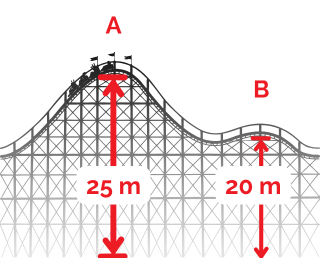
\includegraphics[width=0.22\textwidth]{images/montagne_russe_2.png}
\end{wrapfigure}
Un carrello delle montagne russe di massa $m = 350\ \text{kg}$ scende dal punto A, posto a quota $h_A = 25\ \text{m}$, con velocità iniziale $v_A = 1{,}20\ \text{m/s}$. Il binario è privo di attrito.
\begin{enumerate}
    \item Determina la velocità nel punto B, a quota $h_B = 20\ \text{m}$.
    \item Calcola l'altezza massima che il carrello potrebbe raggiungere senza propulsione.
\end{enumerate}
\begin{solution}
\begin{enumerate}
    \item Conservando l'energia meccanica tra A e B, la diminuzione di quota fornisce energia cinetica aggiuntiva:
    \[
    v_B = \sqrt{v_A^2 + 2g(h_A - h_B)} = \sqrt{1{,}44 + 2\cdot 9{,}81\cdot 5} = \sqrt{99{,}5} \approx \mathbf{9{,}97\ \text{m/s}}.
    \]
    \item L'altezza massima si raggiunge dove la velocità si annulla; tutta l'energia cinetica iniziale in A si converte in potenziale:
    \[
    h_{max} = h_A + \frac{v_A^2}{2g} = 25 + \frac{1{,}44}{19{,}62} \approx \mathbf{25{,}07\ \text{m}}.
    \]
    Il contributo della velocità iniziale è minimo: l'altezza di partenza è quasi il massimo possibile.
\end{enumerate}
\end{solution}
\end{question}

%-----------------------------------------------%

\begin{question}[ID=3.4, subtitle={Molla che spinge un blocco su piano con attrito}, tags={conservazione energia, molla, attrito}, difficulty=media]
Una molla di costante elastica $k = 250\ \text{N/m}$, compressa di $x = 0{,}18\ \text{m}$, spinge un blocco di massa $m = 1{,}5\ \text{kg}$ su un piano orizzontale con coefficiente d'attrito dinamico $\mu_d = 0{,}15$. Il blocco percorre in totale $d = 2{,}3\ \text{m}$ prima di fermarsi.
\begin{enumerate}
    \item Determina l'energia immagazzinata nella molla.
    \item Calcola il lavoro dell'attrito sull'intero percorso.
    \item Determina la velocità del blocco nell'istante in cui la molla raggiunge la lunghezza naturale.
\end{enumerate}
\begin{solution}
\begin{enumerate}
    \item L'energia potenziale elastica accumulata nella molla compressa è
    \[
    E_{molla} = \tfrac{1}{2}kx^2 = \tfrac{1}{2}\cdot 250\cdot (0{,}18)^2 = \mathbf{4{,}05\ \text{J}}.
    \]
    \item L'attrito dinamico è costante ($f = \mu_d mg$) e compie lavoro negativo su tutto il percorso:
    \[
    W_{attrito} = -\mu_d\,m\,g\,d = -0{,}15\cdot 1{,}5\cdot 9{,}81\cdot 2{,}3 \approx \mathbf{-5{,}08\ \text{J}}.
    \]
    \item Quando la molla torna a lunghezza naturale, il blocco ha percorso il solo tratto $x = 0{,}18\ \text{m}$, su cui l'attrito ha sottratto $\mu_d mg\,x = 0{,}397\ \text{J}$. L'energia cinetica disponibile è perciò $E_k = 4{,}05 - 0{,}397 = 3{,}65\ \text{J}$, da cui
    \[
    v = \sqrt{\frac{2E_k}{m}} = \sqrt{\frac{2\cdot 3{,}65}{1{,}5}} \approx \mathbf{2{,}21\ \text{m/s}}.
    \]
\end{enumerate}
\end{solution}
\end{question}

%-----------------------------------------------%

\begin{question}[ID=3.5, subtitle={Moto in potenziale gravitazionale modificato U(x) = mgx + 5x²}, tags={conservazione energia, potenziale}, difficulty=difficile]
Un oggetto di massa $m = 0{,}3\ \text{kg}$ si muove in una regione in cui l'energia potenziale è $U(x) = mgx + 5x^2$ (in joule, con $x$ in metri). In $x = 0$ ha velocità $v_0 = 3\ \text{m/s}$.
\begin{enumerate}
    \item Determina la velocità in $x = 0{,}4\ \text{m}$.
    \item Determina il punto di inversione $x_{max}$.
    \item Stabilisci se l'oggetto può superare la barriera situata oltre $x = 1\ \text{m}$.
\end{enumerate}
\begin{solution}
L'energia meccanica totale si conserva. In $x = 0$ è $U(0) = 0$, quindi
\[
E_{tot} = \tfrac{1}{2}mv_0^2 = \tfrac{1}{2}\cdot 0{,}3\cdot 9 = 1{,}35\ \text{J}.
\]
\begin{enumerate}
    \item In $x = 0{,}4\ \text{m}$ il potenziale vale
    \[
    U(0{,}4) = 0{,}3\cdot 9{,}81\cdot 0{,}4 + 5\cdot 0{,}16 = 1{,}18 + 0{,}80 = 1{,}98\ \text{J} > E_{tot}.
    \]
    Poiché servirebbe più energia di quella disponibile, l'oggetto \textbf{non raggiunge} $x = 0{,}4\ \text{m}$.
    \item Il punto di inversione è dove tutta l'energia diventa potenziale, $U(x_{max}) = E_{tot}$:
    \[
    2{,}943\,x + 5x^2 = 1{,}35 \;\Rightarrow\; x_{max} \approx \mathbf{0{,}30\ \text{m}}.
    \]
    \item In $x = 1\ \text{m}$ il potenziale $U(1) = 0{,}3\cdot 9{,}81 + 5 = 7{,}94\ \text{J} \gg E_{tot}$: la barriera è troppo alta e l'oggetto \textbf{non la supera}.
\end{enumerate}
\end{solution}
\end{question}

%====================================================%
% SEZIONE 4: FORZE NON CONSERVATIVE
%====================================================%

\begin{question}[ID=4.1, subtitle={Carrellino su piano inclinato con tratto orizzontale scabro}, tags={conservazione energia, forze non conservative, attrito}, difficulty=media]
\begin{wrapfigure}{r}{0.3\textwidth}
\vspace{-20pt}
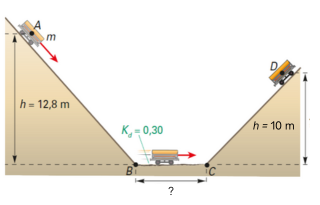
\includegraphics[width=\linewidth]{images/discesa_scabra.png}
\end{wrapfigure}
Un carrellino di massa $m = 1\ \text{kg}$ parte da A (altezza $12{,}8\ \text{m}$) lungo un tratto liscio, percorre il tratto orizzontale scabro BC con coefficiente d'attrito $\mu_d = 0{,}30$, e infine risale, senza attrito, fino a un'altezza di $10\ \text{m}$.
\begin{enumerate}
    \item Determina il lavoro delle forze non conservative lungo BC.
    \item Calcola la lunghezza del tratto BC.
\end{enumerate}
\begin{solution}
\begin{enumerate}
    \item I tratti in salita e discesa sono lisci, quindi l'energia meccanica si perde solo lungo BC. Il lavoro delle forze non conservative è pari alla variazione di energia meccanica tra partenza e arrivo (entrambe a velocità nulla):
    \[
    W_{nc} = \Delta E_{mec} = mg(h_f - h_i) = 1\cdot 9{,}81\cdot(10 - 12{,}8) = \mathbf{-27{,}5\ \text{J}}.
    \]
    \item Questo lavoro è quello dell'attrito lungo BC, $|W_{nc}| = \mu_d\,m\,g\,L_{BC}$, da cui
    \[
    L_{BC} = \frac{|W_{nc}|}{\mu_d\,m\,g} = \frac{27{,}5}{0{,}30\cdot 9{,}81} \approx \mathbf{9{,}3\ \text{m}}.
    \]
\end{enumerate}
\end{solution}
\end{question}


%====================================================%
% SEZIONE 5: MISCELLANEA
%====================================================%
\begin{question}[ID=5.1, subtitle={Pendolo con piolo — velocità al punto più alto}, tags={conservazione energia, pendolo}, difficulty=media]
\begin{wrapfigure}{r}{0.3\textwidth}
\vspace{-40pt}
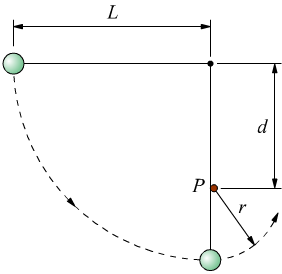
\includegraphics[width=\linewidth]{images/pendolo_piolo.png}
\end{wrapfigure}
Una massa è collegata a una corda di lunghezza $L = 130\ \text{cm}$ vincolata a una cerniera. Un piolo P dista $d = 75\ \text{cm}$ dalla cerniera. La massa parte ferma in posizione orizzontale; durante l'oscillazione la corda si impiglia nel piolo e la massa prosegue ruotando attorno a esso. Determina la velocità nel punto più alto dell'arco attorno al piolo.
\begin{solution}
Quando la corda si impiglia, il raggio della traiettoria diventa $r = L - d = 55\ \text{cm} = 0{,}55\ \text{m}$. Il punto più alto di questo arco si trova a quota
\[
h_f = -d + r = -0{,}75 + 0{,}55 = -0{,}20\ \text{m}
\]
rispetto alla cerniera (presa come riferimento $h_i = 0$, dato che la massa parte in posizione orizzontale).

Conservando l'energia meccanica tra la partenza e il punto più alto, la massa è scesa complessivamente di $|h_f| = 0{,}20\ \text{m}$:
\[
v = \sqrt{2g\,|h_f|} = \sqrt{2\cdot 9{,}81\cdot 0{,}20} \approx \mathbf{1{,}98\ \text{m/s}}.
\]
\end{solution}
\end{question}

%====================================================%
% SEZIONE FAC
%====================================================%
\begin{question}[ID=fac.1, subtitle={Due molle: quante volte il blocco urta le pareti?}, tags={conservazione energia, molla, attrito}, difficulty=difficile]
\textbf{FAC.}\\
Due molle identiche ($k = 5000\ \text{N/m}$) sono fissate a due pareti parallele, con le estremità libere distanti $1\ \text{m}$. Un blocco di massa $m = 0{,}5\ \text{kg}$ comprime la prima molla di $10\ \text{cm}$ e viene rilasciato su un piano con coefficiente d'attrito $\mu_d = 0{,}01$. Quante volte il blocco urta le due molle prima di fermarsi definitivamente?
\begin{solution}
L'energia inizialmente immagazzinata nella molla compressa è
\[
E_0 = \tfrac{1}{2}kx^2 = \tfrac{1}{2}\cdot 5000\cdot (0{,}10)^2 = 25\ \text{J}.
\]
A ogni traversata da una parete all'altra (percorso $\approx 1\ \text{m}$) l'attrito sottrae una quantità fissa di energia:
\[
\Delta E = \mu_d\,m\,g\,d = 0{,}01\cdot 0{,}5\cdot 9{,}81\cdot 1 \approx 0{,}049\ \text{J per traversata}.
\]
Il numero di traversate possibili prima dell'arresto è
\[
n = \frac{E_0}{\Delta E} = \frac{25}{0{,}049} \approx 510.
\]
Ogni traversata termina con un urto contro una molla, quindi il blocco urta le due molle circa $\mathbf{510}$ volte in totale (all'incirca $255$ contro ciascuna).
\end{solution}
\end{question}
